\subsection{Backend}
{\tiny Written by: Sven}

\subsection{Backend Implementation}

This subsection provides an overview of the implementation details for the backend of the locker system. It covers the technologies, frameworks, and development environment used in the development process.

\subsubsection{Project Setup}

The backend part of the locker system project is developed using FastAPI and SQLAlchemy/alembic. These technologies were chosen for their robustness, scalability, and ease of use in building web APIs and managing database migrations.

The development environment setup involves several steps to ensure a smooth workflow. Firstly, it requires a local Postgres database instance to be running, with specific configuration settings provided via environment variables. These variables include the database username, password, host, port, and name.

The project setup also involves cloning the backend repository and configuring the environment variables as necessary. A virtual environment is then created to isolate dependencies, followed by the installation of required packages specified in the `requirements.txt` file using pip.

Once the development environment is set up, the application can be run locally by activating the virtual environment and starting the application. Additionally, database migrations can be managed using alembic, with commands provided to generate and apply migration scripts.

\subsubsection{List of Important Libraries and Versions}

The following list includes the most important libraries used in the backend implementation along with their versions:

\begin{itemize}
    \item \textbf{FastAPI} (\texttt{fastapi==0.110.2}): FastAPI is a modern, fast (high-performance) web framework for building APIs with Python 3.7+ based on standard Python type hints.

    \item \textbf{SQLAlchemy} (\texttt{SQLAlchemy==2.0.29}): SQLAlchemy is the Python SQL toolkit and Object-Relational Mapper that gives application developers the full power and flexibility of SQL.

    \item \textbf{Alembic} (\texttt{alembic==1.13.1}): Alembic is a lightweight database migration tool for usage with the SQLAlchemy Database Toolkit for Python.

    \item \textbf{Pydantic} (\texttt{pydantic==2.7.1}): Pydantic is a data validation and settings management using Python type annotations.

    \item \textbf{uvicorn} (\texttt{uvicorn==0.29.0}): Uvicorn is a lightning-fast ASGI server implementation, using uvloop and httptools.

    \item \textbf{psycopg2-binary}: Psycopg is the most popular PostgreSQL database adapter for the Python programming language.
\end{itemize}

\subsubsection{Request Handling in FastAPI and SQLAlchemy}

A crucial aspect of understanding the backend implementation is to grasp how FastAPI and SQLAlchemy handle incoming requests and interact with the database. The following diagram illustrates the request handling process:

\begin{figure}[h]
    \centering
    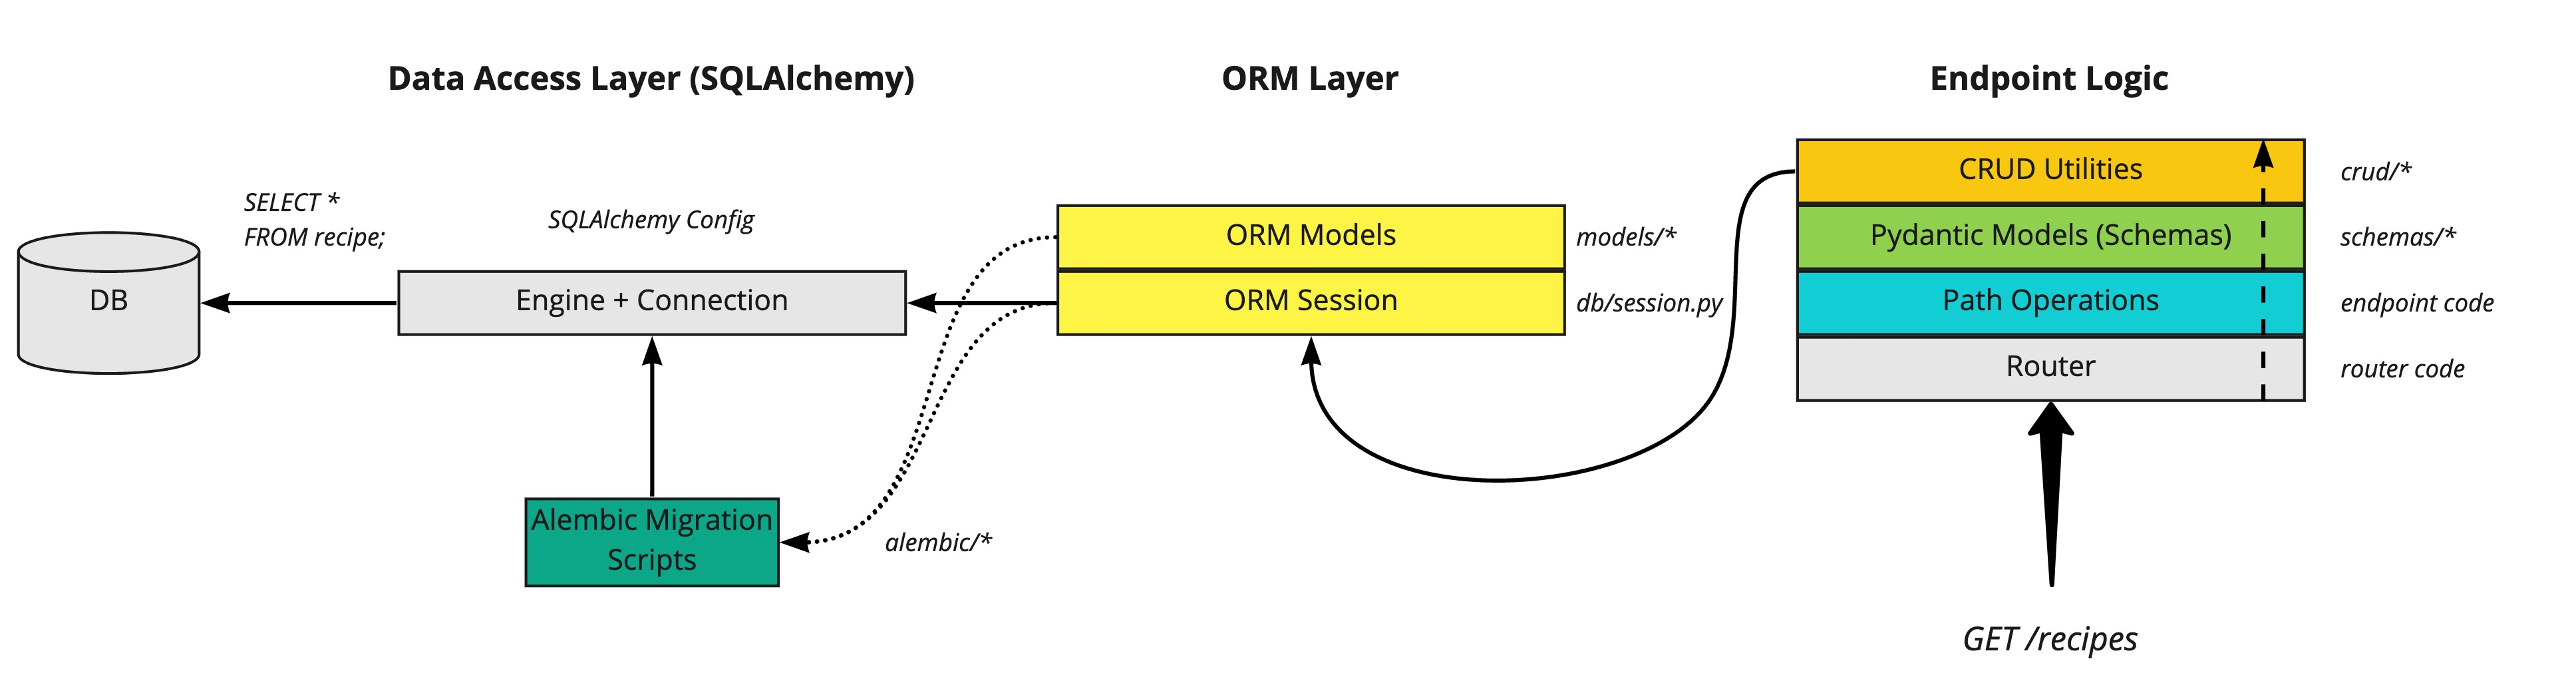
\includegraphics[width=0.8\textwidth]{images/request_handling_diagram}
    \caption{Request Handling in FastAPI and SQLAlchemy \citet{samiullah_fastapi_tutorial}}
    \label{fig:request_handling}
\end{figure}


This diagram visually depicts the sequence of steps involved in processing a client request, starting from the client making an HTTP request to the backend API. FastAPI routes the request to the appropriate endpoint, where it is processed by the corresponding router function. The router function interacts with the database through SQLAlchemy ORM, executing CRUD operations as necessary to fulfill the request. Once the database operations are complete, a response is generated and returned to the client.

Understanding this request handling flow is essential for developers to comprehend the inner workings of the backend system and troubleshoot any issues that may arise during development or deployment.


\subsubsection{Project Structure}

The backend part of the locker system project adheres to a well-organized structure, following best practices to ensure clarity, modularity, and maintainability. Below is an overview of the project structure and the rationale behind each component:

\begin{itemize}
    \item \textbf{README.md}: This file serves as the project's main documentation hub, containing comprehensive information on setup instructions, deployment steps, and other essential details. A well-written README enhances project understanding and facilitates collaboration among team members.

    \item \textbf{requirements.txt}: This file enumerates all Python packages required by the project, making it easy for developers to install dependencies using pip. Managing dependencies in a centralized file promotes consistency and reproducibility across different environments.

    \item \textbf{.env}: Environment variables play a crucial role in configuring the application, especially sensitive information like database credentials. Utilizing a separate .env file allows for easy management of configuration settings across various deployment environments.

    \item \textbf{venv}: The virtual environment isolates project dependencies, ensuring compatibility and preventing conflicts with other Python projects. By encapsulating dependencies within a dedicated environment, developers can maintain a clean and reproducible development setup.

    \item \textbf{alembic/versions}: This directory houses database migration files managed by Alembic, a lightweight migration tool for SQLAlchemy. Organizing migrations in a structured manner facilitates version control and systematic evolution of the database schema over time.

    \item \textbf{images}: Images used in the project documentation, such as the README file, are stored in this directory. Including visual aids enhances readability and comprehension of project-related instructions and guidelines.

    \item \textbf{Dockerfile}: Docker simplifies application deployment by encapsulating the application and its dependencies into portable containers. The Dockerfile specifies the steps to build a Docker image, promoting consistency and reproducibility across different deployment environments.
\end{itemize}

The \textbf{app} folder encapsulates the core components of the backend application. It is further divided into the following subdirectories and files (examples are used from the Category class, but the structure is the same for all classes):

\begin{itemize}
    \item \textbf{api} folder: This folder contains endpoint-specific modules responsible for handling HTTP requests and responses. Each endpoint module typically consists of three main components:

    \begin{itemize}
        \item \textbf{CRUD operations (Create, Read, Update, Delete)}: These operations define the basic functionalities for interacting with database entities. For example, the \texttt{crud.py} files contain functions for creating, retrieving, updating, and deleting records from the database.

        The following code snippet demonstrates the \texttt{delete\_category\_by\_id} function, which is responsible for deleting a category from the database by its ID:

        \begin{lstlisting}[language=Python]
        def delete_category_by_id(category_id: int, db: Session):
            category = get_category_by_id(category_id, db)
            if category:
                db.delete(category)
                db.commit()
        \end{lstlisting}

        This function first retrieves the category with the specified ID using the \texttt{get\_category\_by\_id} function. If the category exists, it is deleted from the database using the SQLAlchemy \texttt{delete} method, followed by a commit to persist the changes.


        \item \textbf{Router functions}: The \texttt{router.py} files define FastAPI router instances responsible for routing HTTP requests to the appropriate endpoint functions. Routers enhance code organization and modularity by grouping related endpoint operations together.

        The following code snippet illustrates a router function responsible for handling HTTP DELETE requests to delete a category:

        \begin{lstlisting}[language=Python]
        @router.delete('/categories/{category_id}', response_model=None, tags=['category'])
        def delete_category(
                category_id: int,
                db: Session = Depends(get_db)):
            category_crud.delete_category_by_id(category_id, db)
            return Response(status_code=status.HTTP_204_NO_CONTENT)
        \end{lstlisting}

        In this function, the route decorator specifies the HTTP method (DELETE) and the endpoint URL pattern ("/categories/{category\_id}"). The function parameters include the category ID to be deleted and a database session dependency obtained through the \texttt{get\_db} function. Inside the function, the \texttt{delete\_category\_by\_id} function from the CRUD module (\texttt{category\_crud}) is called to delete the category from the database. Finally, a 204 No Content response is returned to indicate successful deletion.


        \item \textbf{Schema definitions}: Schemas define the structure and validation rules for request and response payloads exchanged between the client and server. The \texttt{schemas.py} files contain Pydantic models representing data schemas for serialization and validation purposes.

        The following code snippet presents a Pydantic model (\texttt{CategoryBaseSchema}) defined in a schema file:

        \begin{lstlisting}[language=Python]
        class CategoryBaseSchema(BaseModel):
            name: str
        \end{lstlisting}

        In this schema definition, \texttt{CategoryBaseSchema} inherits from \texttt{BaseModel}, a Pydantic base class used for defining data models. The schema consists of a single field (\texttt{name}) with a data type of \texttt{str}, representing the name of a category. Pydantic models provide automatic data validation based on the specified field types, enabling robust input validation and serialization/deserialization of data between client and server components.

    \end{itemize}

    \item \textbf{db} folder: This folder contains modules related to database management and configuration. Key components include:

    \begin{itemize}
        \item \textbf{Configuration module (\texttt{config.py})}: This module defines database connection settings using environment variables and provides functions for establishing database connections and checking connectivity status. Centralizing database configuration facilitates easy maintenance and deployment across different environments.

        The following code snippet illustrates the \texttt{config.py} module, which manages database configuration:

        \begin{lstlisting}[language=Python]
        from sqlalchemy import create_engine
        from sqlalchemy.orm import sessionmaker
        from sqlalchemy.exc import OperationalError
        from dotenv import load_dotenv
        import os

        load_dotenv()

        DB_USERNAME = os.getenv("DATABASE_USERNAME")
        DB_PASSWORD = os.getenv("DATABASE_PASSWORD")
        DB_HOST = os.getenv("DATABASE_HOST")
        DB_PORT = os.getenv("DATABASE_PORT")
        DB_NAME = os.getenv("DATABASE_NAME")
        DB_URL = f"postgresql://{DB_USERNAME}:{DB_PASSWORD}@{DB_HOST}:{DB_PORT}/{DB_NAME}"

        def get_database_url():
            return DB_URL

        engine = create_engine(DB_URL)
        SessionLocal = sessionmaker(autocommit=False, autoflush=False, bind=engine)

        def check_database_connection():
            try:
                engine = create_engine(DB_URL)
                with engine.connect():
                    return True
            except OperationalError:
                return False
        \end{lstlisting}

        This module loads database connection settings from environment variables using the \texttt{dotenv} library. It defines functions for retrieving the database URL, establishing a database engine, and checking database connectivity. By encapsulating database configuration in a single module, the codebase becomes more modular and maintainable, enabling seamless deployment across various environments.


        \item \textbf{Model definitions (\texttt{models.py})}: Models define the structure of database tables and their relationships using SQLAlchemy declarative base. Models encapsulate business logic and data integrity constraints, promoting code organization and reusability.

        The following code snippet demonstrates a model definition (\texttt{Category}) in the \texttt{models.py} module:

        \begin{lstlisting}[language=Python]
        from sqlalchemy import Column, Integer, String
        from db.config import Base

        class Category(Base):
            __tablename__ = 'categories'

            id = Column(Integer, primary_key=True)
            name = Column(String, nullable=False)
        \end{lstlisting}

        In this model definition, \texttt{Category} is a SQLAlchemy model representing the \texttt{categories} table in the database. It inherits from \texttt{Base}, the declarative base provided by SQLAlchemy. The \texttt{\_\_tablename\_\_} attribute specifies the table name, while \texttt{id} and \texttt{name} represent the table columns. By encapsulating database schema in model classes, the codebase becomes more organized and maintainable, facilitating data manipulation and ensuring data integrity.
    \end{itemize}

    \item \textbf{main.py}: The main entry point of the backend application, responsible for initializing the FastAPI application instance and configuring middleware, routers, and other application-level settings.
\end{itemize}

\subsubsection{API Design}

The backend API is documented using the OpenAPI Specification (OAS) format, commonly known as Swagger. Swagger provides a standardized, machine-readable representation of the API, detailing its endpoints, request/response formats, and data models.

\textbf{What is Swagger?}:
Swagger is an open-source framework that enables the design, documentation, and testing of RESTful APIs. It defines a structured format for describing API endpoints, parameters, responses, and authentication mechanisms, facilitating seamless integration and collaboration among developers.

\begin{figure}[h]
    \centering
    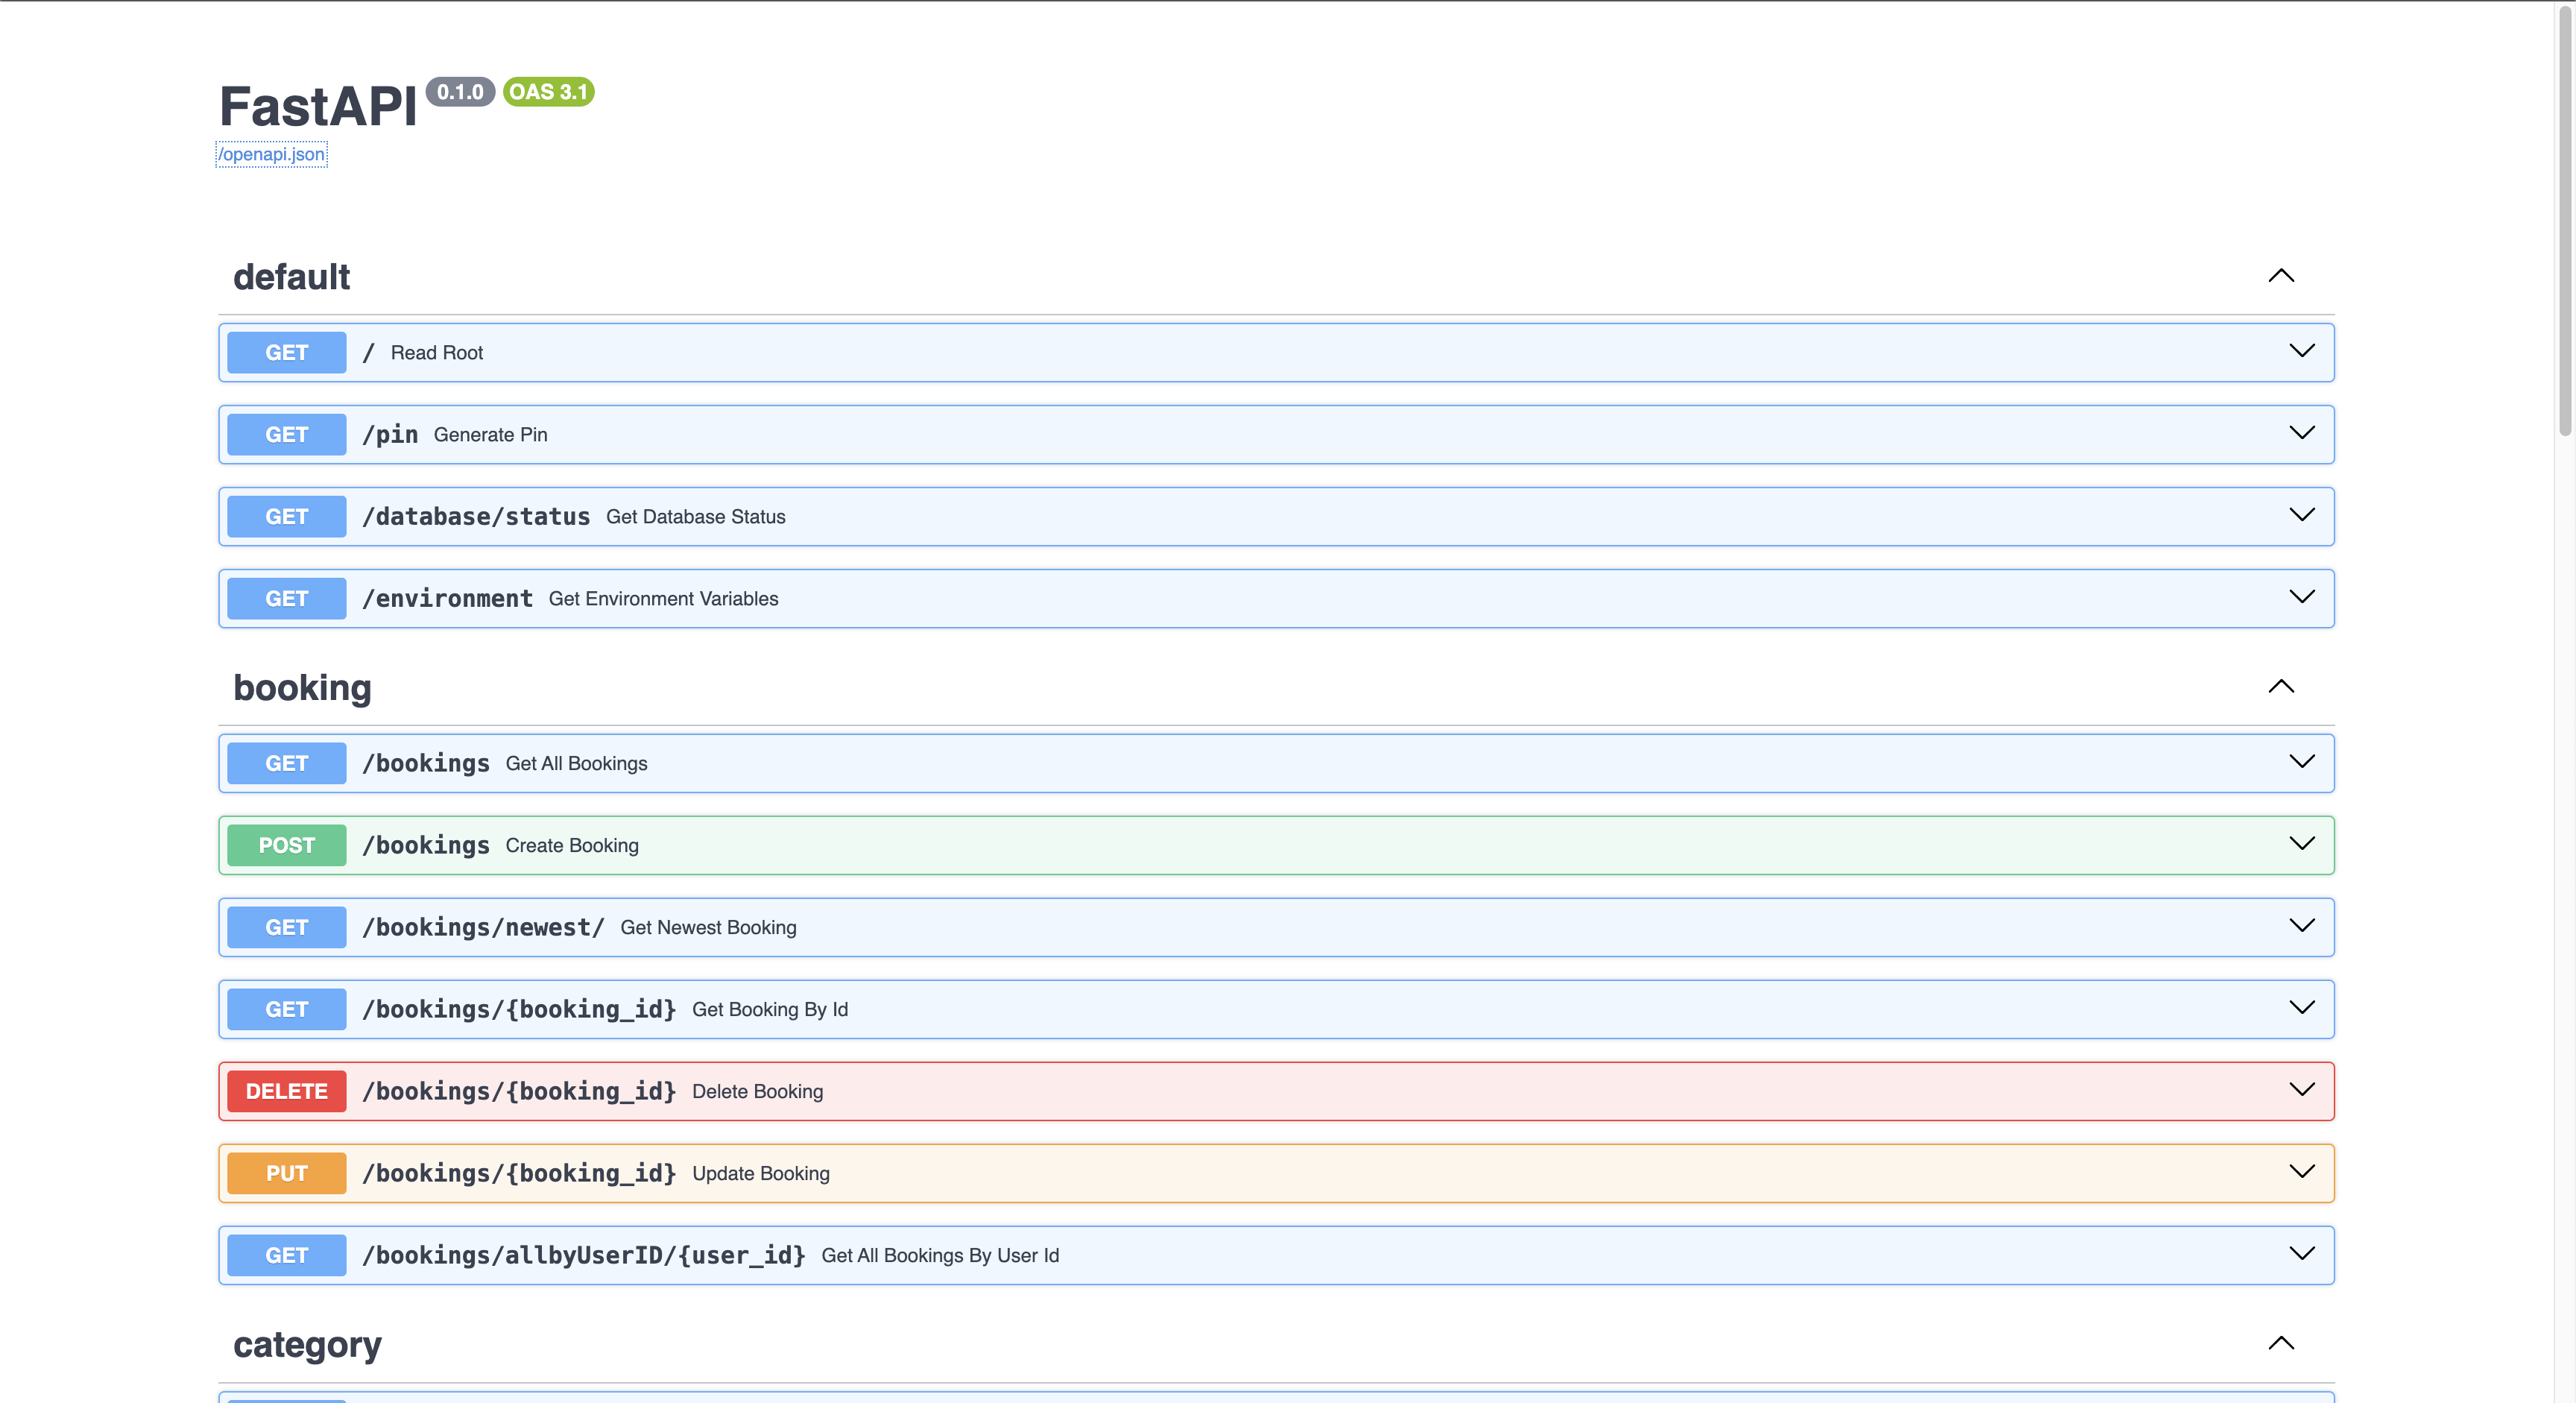
\includegraphics[width=0.8\textwidth]{images/swagger_ui}
    \caption{FastAPI Swagger UI}
    \label{fig:swagger_ui}
\end{figure}

\textbf{Why is Swagger Useful?}:
Swagger simplifies API development by offering a centralized platform for describing and visualizing API specifications. It enhances communication between frontend and backend developers, accelerates client-side integration, and fosters interoperability across diverse programming languages and frameworks.

\textbf{FastAPI and Swagger}:
FastAPI, a modern web framework for building APIs with Python, integrates seamlessly with Swagger to automate API documentation. FastAPI generates Swagger UI out of the box, allowing developers to interactively explore and test API endpoints. By leveraging FastAPI's native support for Swagger, developers can focus on implementing business logic without worrying about manual documentation efforts.

\textbf{Endpoints Definition}:
The backend API comprises a set of well-defined endpoints, each catering to a specific functionality within the locker system. Endpoints such as \texttt{/bookings}, \texttt{/categories}, \texttt{/devices}, \texttt{/reports}, \texttt{/users}, among others, provide access to the corresponding resources and operations.

\begin{figure}[h]
    \centering
    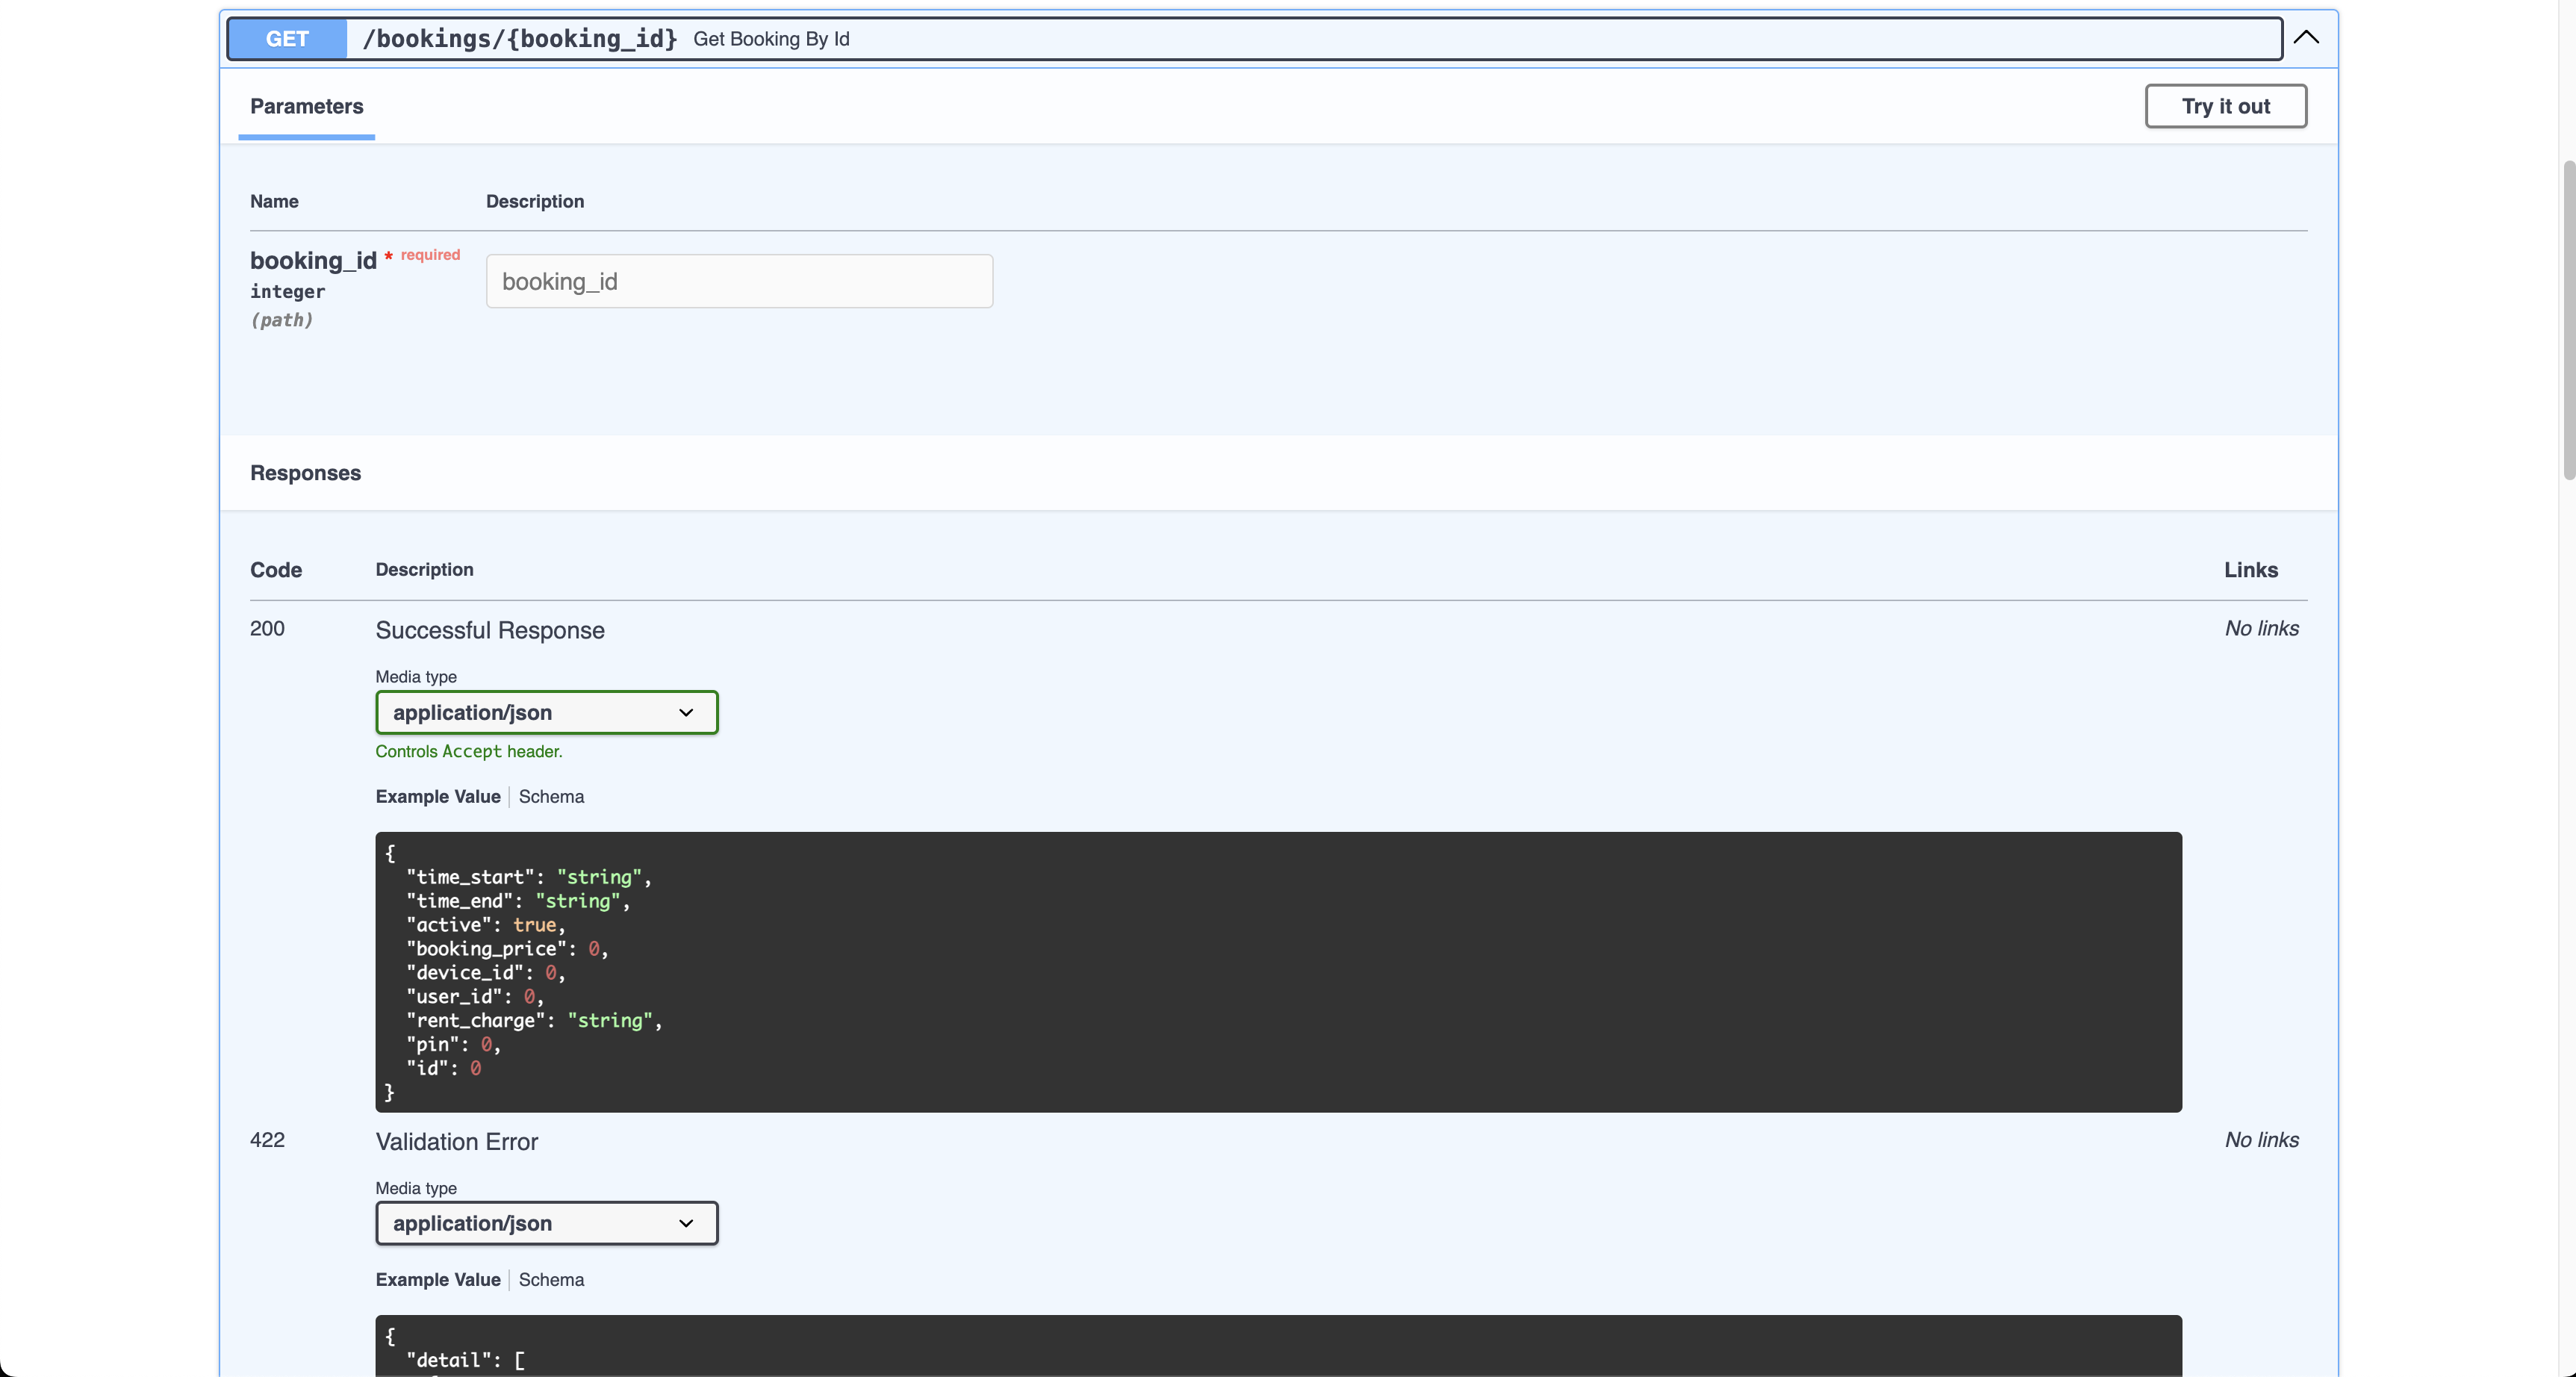
\includegraphics[width=0.8\textwidth]{images/swagger_ui_bookings}
    \caption{FastAPI Swagger UI - Bookings Endpoint}
    \label{fig:swagger_ui_bookings}
\end{figure}

\textbf{Request/Response Formats}:
For each endpoint, clear specifications are provided regarding the expected request formats, including request bodies, query parameters, and path parameters. Similarly, the response formats, denoted by response schemas, outline the structure of data returned by the server in response to client requests.

\textbf{Data Models}:
The API leverages distinct data models to represent various entities and their attributes. These models, including \texttt{BookingSchema}, \texttt{CategorySchema}, \texttt{DeviceSchema}, \texttt{ReportSchema}, and \texttt{UserSchema}, encapsulate the structure of data exchanged between the client and server. Additionally, specialized schemas such as \texttt{BookingCreateSchema}, \texttt{CategoryCreateSchema}, and others are utilized for specific operations, ensuring consistency and validation of incoming data.

\subsubsection{Database Schema Design}

The database schema for the locker system is designed to efficiently store information related to bookings, categories, devices, reports, and users. The schema employs normalization techniques to minimize redundancy and ensure data integrity. Indexing strategies are implemented to optimize query performance, particularly for frequently accessed fields.

\begin{figure}[h]
    \centering
    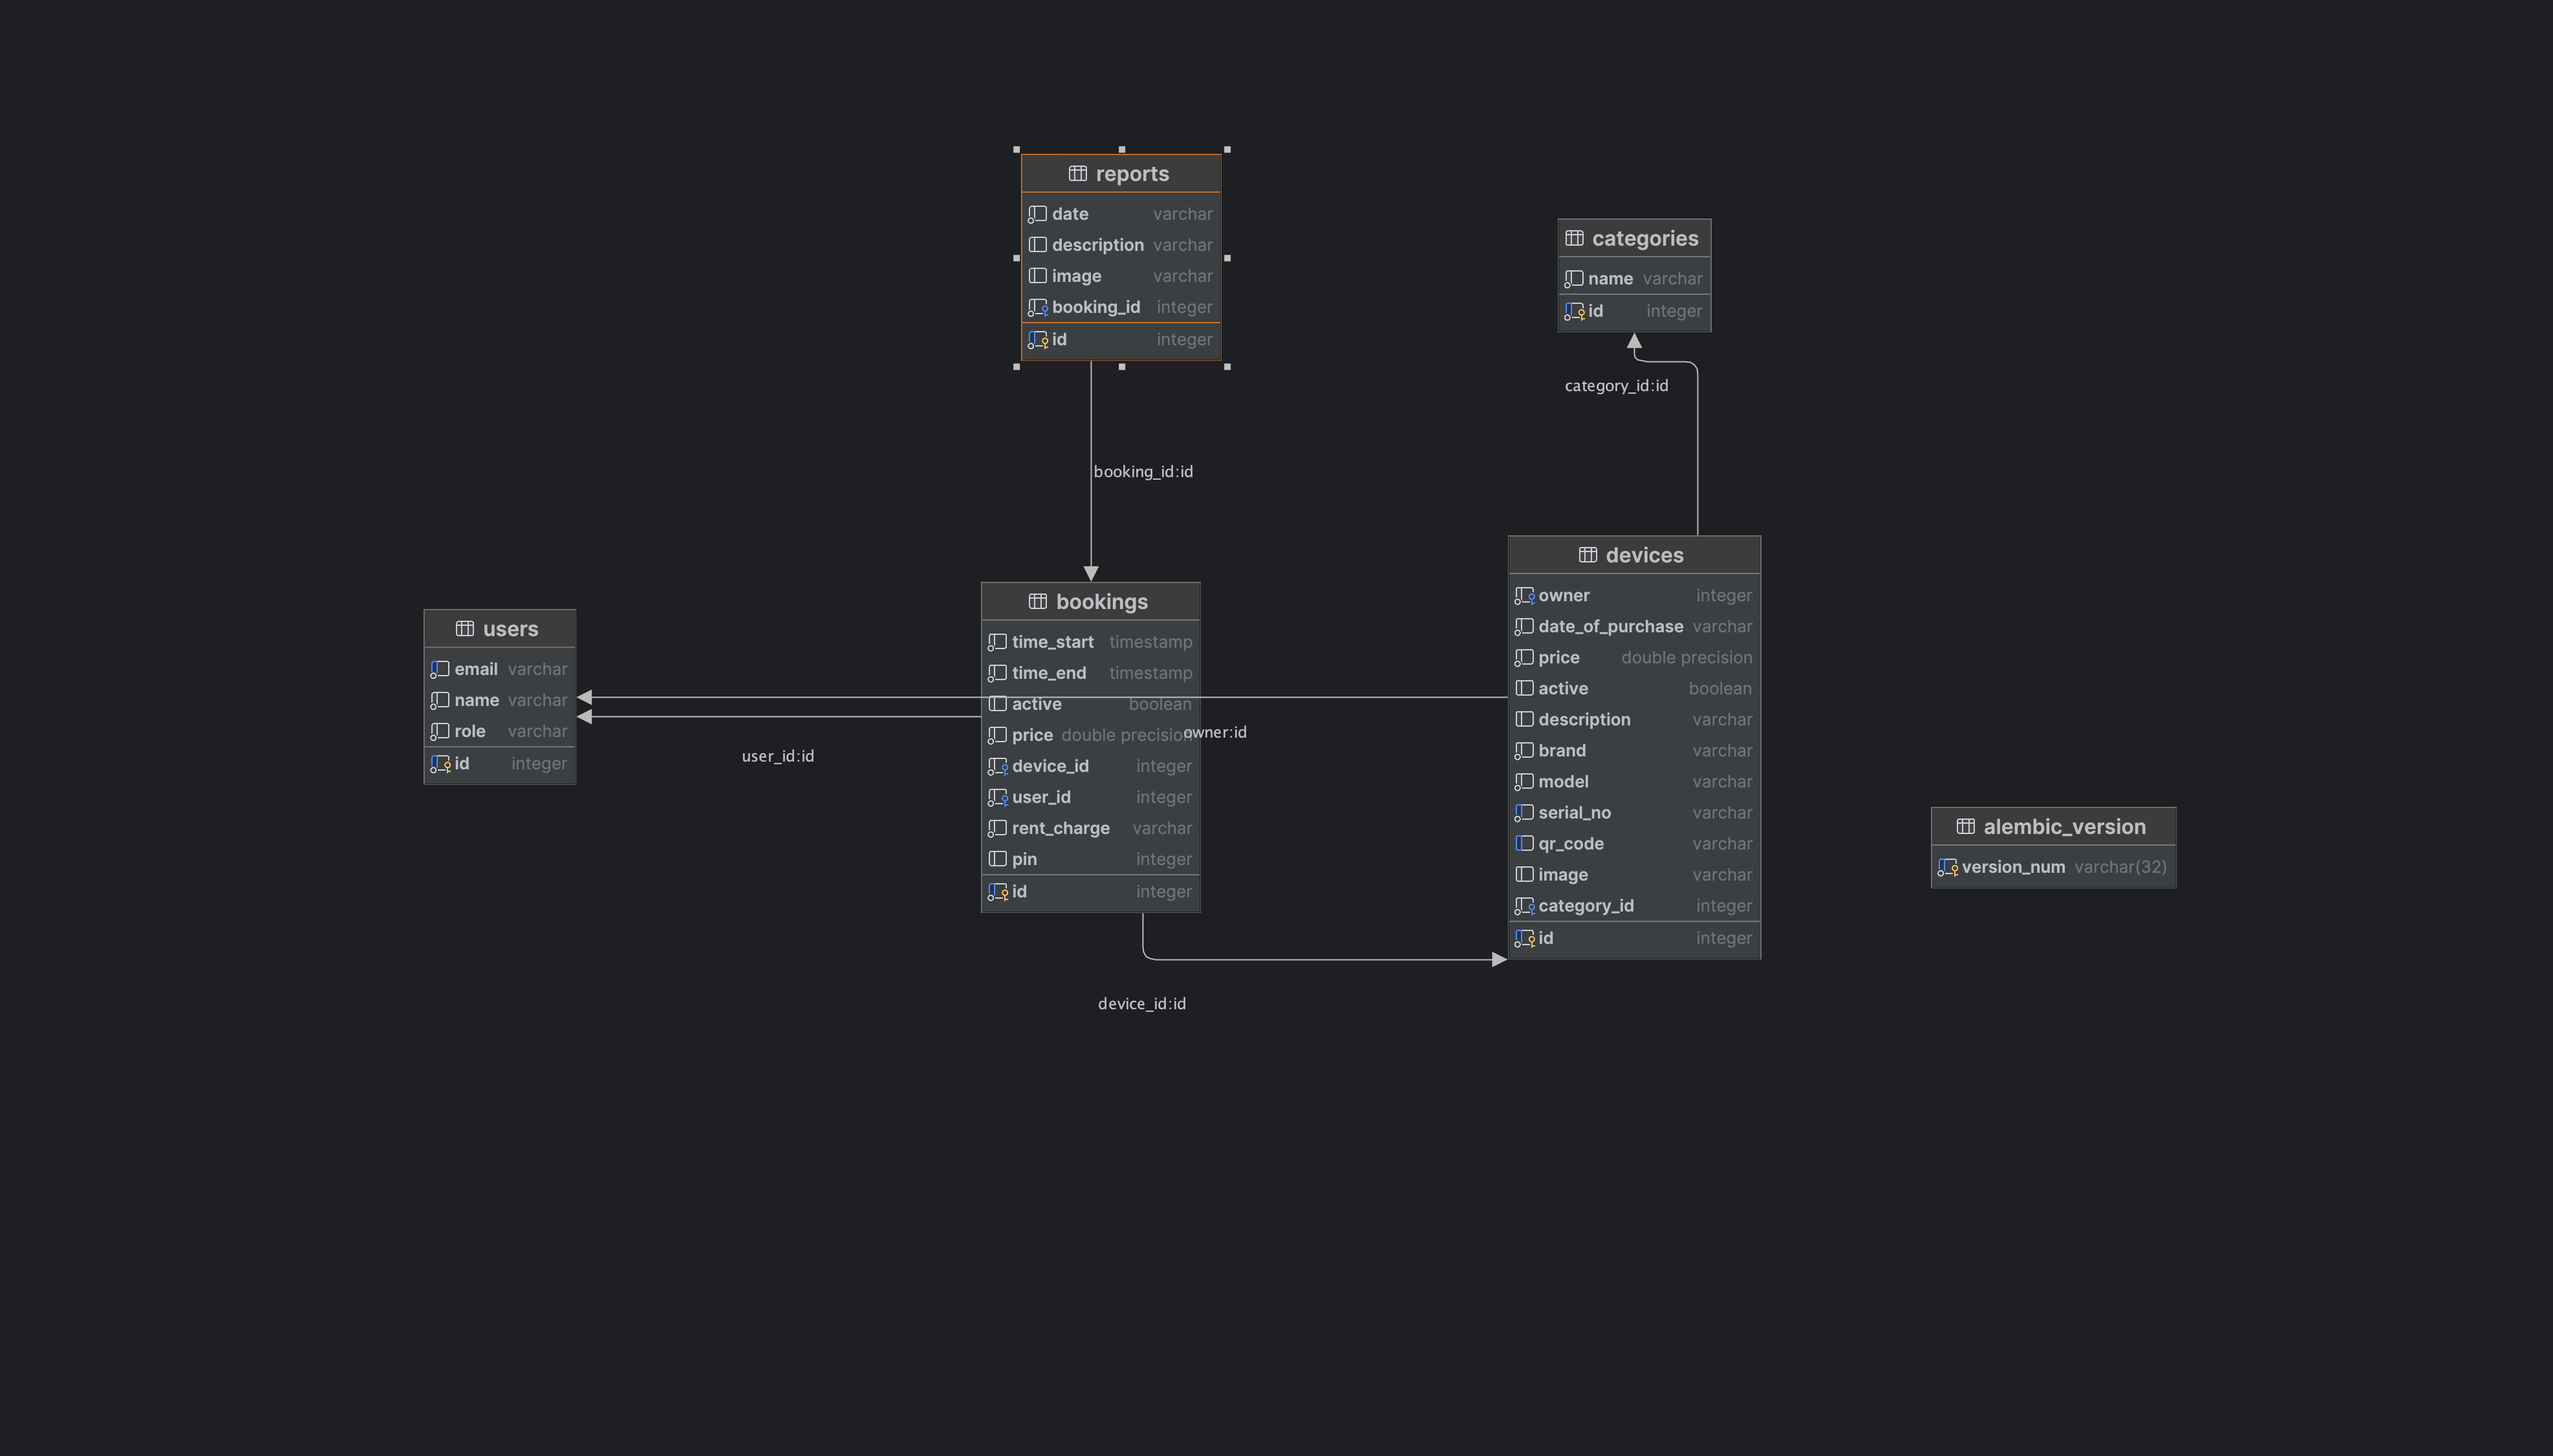
\includegraphics[width=0.8\textwidth]{images/db_schema}
    \caption{Database Schema Design}
    \label{fig:dbschema}
\end{figure}

\textbf{Normalization}:
The schema adheres to normalization principles to eliminate data redundancy and dependency issues. By organizing data into well-structured tables and establishing relationships between them, normalization ensures efficient data storage and maintenance.

\textbf{Indexing}:
To enhance query performance, the database schema incorporates appropriate indexes on key fields. Indexing accelerates data retrieval operations by facilitating quick access to specific records, especially in scenarios involving large datasets.

\textbf{Optimization}:
The schema design incorporates optimization strategies to streamline database operations and enhance overall system performance. Techniques such as query optimization, caching, and resource allocation are employed to mitigate bottlenecks and ensure optimal resource utilization.

\subsubsection{Logging}

Logging plays a crucial role in monitoring and troubleshooting the backend operations of the locker system. By capturing relevant information during runtime, logging enables developers to track system behavior, identify errors, and analyze performance metrics.

\textbf{Logging Implementation}:
The backend API incorporates logging functionality to record significant events and activities. The Python logging module provides a flexible framework for logging messages of varying severity levels to different destinations, including files, streams, or external services.

\textbf{Example:} Consider the following function for creating a booking within the locker system:

\begin{lstlisting}[language=Python]
def create_booking(schema: BookingCreateSchema, db: Session):
    entity = Booking(**schema.dict())
    entity.pin = random.randint(1000, 9999)
    logging.info('Booking created with id {}'.format(entity.id))
    db.add(entity)
    db.commit()
    return entity
\end{lstlisting}

In this example, the \texttt{create\_booking} function creates a new booking entity based on the provided schema. After generating a random PIN for the booking, the function logs a message indicating the successful creation of the booking along with its ID. This logging statement provides valuable insights into the system's activity and facilitates debugging and auditing processes.

\subsubsection{Areas for Improvement}

While the backend implementation of the locker system prototype adheres to common best practices, several areas require further attention and refinement before the system can be considered production-ready:

\begin{itemize}
    \item \textbf{Error Handling}: The current implementation lacks comprehensive error handling mechanisms, which are essential for gracefully managing unexpected scenarios and providing informative feedback to users. For example, enhancing error responses with appropriate status codes and error messages would improve the system's robustness.

    \item \textbf{Infrastructure}: The prototype operates in a development environment and lacks the infrastructure necessary for deployment in a production setting. Implementing scalable infrastructure components, such as load balancers, auto-scaling groups, and fault-tolerant databases, is crucial for ensuring system reliability and performance under varying workloads.

    \item \textbf{Validation}: While basic input validation is incorporated into the API endpoints, there is room for strengthening validation logic to enforce data integrity and prevent malicious inputs. Implementing robust validation mechanisms, such as input sanitization and parameter validation, would enhance the security and reliability of the system.

    \item \textbf{Security}: Security measures, including authentication, authorization, and data encryption, are fundamental requirements for safeguarding sensitive information and protecting the system against security threats. Implementing authentication mechanisms, role-based access control (RBAC), and encryption protocols would mitigate security risks and enhance the system's trustworthiness.
\end{itemize}

Addressing these areas of improvement would contribute to the development of a robust, secure, and scalable backend system for the locker application.


